%!TEX program = xelatex


\documentclass[aspectratio=169]{beamer}
%\documentclass{beamer}

\usepackage{blindtext}

\usepackage{beamerthemeFeecBUT}

\usepackage{xltxtra}
\usepackage[export]{adjustbox}

\usepackage{amssymb}% http://ctan.org/pkg/amssymb
\usepackage{pifont}% http://ctan.org/pkg/pifont
\newcommand{\cmark}{\ding{51}}%
\newcommand{\xmark}{\ding{55}}%
% \usepackage[paperwidth=29cm, paperheight=15cm]{geometry}
% \usepackage[a5paper, landscape]{geometry}

\defaultfontfeatures{Ligatures=TeX}

\def\checkmark{\tikz\fill[scale=0.4](0,.35) -- (.25,0) -- (1,.7) -- (.25,.15) -- cycle;}

\title{Nástroje pro diagnostiku integrity souborového systému v OS Linux}
\subtitle{Obhajoba diplomové práce}
\author{Bc. Vojtěch Vladyka}
\garant{Ing. Petr Petyovský, Ph.D.}
\date{6.června 2017}

\begin{document}
	\addtolength{\textwidth}{-20pt}
	\addtolength{\textheight}{-20pt}
  \frame{\titlepage}
   
	\section{Úvod}
		\begin{frame}
			\frametitle{Zadání práce}
			\vspace{40 pt}
			\large 
            Cílem práce je vytvořit nástroje pro~diagnostiku integrity dat souborových systémů v~OS~Linux, pro~které v~současnosti tato podpora neexistuje.
            \vspace{10pt}
            \begin{enumerate}
                \item Zvolte vhodný typ souborového systému, pro který nejsou plně implementovány nástroje pro diagnostiku integrity dat.
                \item Navrhněte a vytvořte vlastní nástroje pro diagnostiku chyb zvoleného souborového systému.
                \item Realizujte vlastní nástroje pro opravu chyb v daném souborovém systému.
                \item Integrujte vytvořené nástroje do prostředí OS Linux. Publikujte tyto nástroje GNU komunitě.
                \item Zhodnoťte dosažené výsledky, uveďte výhody a nevýhody řešení a navrhněte další možná rozšíření.
            \end{enumerate}
		\end{frame}
        \begin{frame}
            \frametitle{Nástroje kontroly integrity dat}
            % TODO popsat fsck nástroje a jejich existenci pro FS v Linuxu
            \vspace{40pt}
            \begin{itemize}
                \Large\item Nástoj \texttt{fsck} kontroluje metadata a žurnály souborových systémů v~OS~Linux.
                \Large\item Pro každý souborový systém je tento nástroj \textit{jiný} (obvykle je dodáván s nástroji k souborovému systému) ale je zapouzdřen nástrojem \texttt{fsck}
                \Large\item Integrita sektorů je zajištěna médiem samotným (ECC~bloky) ale souborový systém musí zajistit integritu napříč sektory.
            \end{itemize}
        \end{frame}
        \begin{frame}
            \frametitle{Volba souborového systému}
            % TODO popsat důvody výběru UDF
            \vspace{30pt}
            \huge
            \center
            Při rešerši bylo zjištěno,\\že pro souborový systém \textit{Universal~Disk~Format} tyto nástroje \textbf{chybí}.

            \vspace{30pt} 
            \Large
            Vzhledem k univerzálnosti a perspektivě tohoto souborového systému byl \textbf{vybrán pro další práci}.
        \end{frame}

	\section{Universal Disk Format}
		\begin{frame}
			\frametitle{Vlastnosti souborového systému UDF}
			\vspace{40 pt}
			\center
            \begin{figure}
			    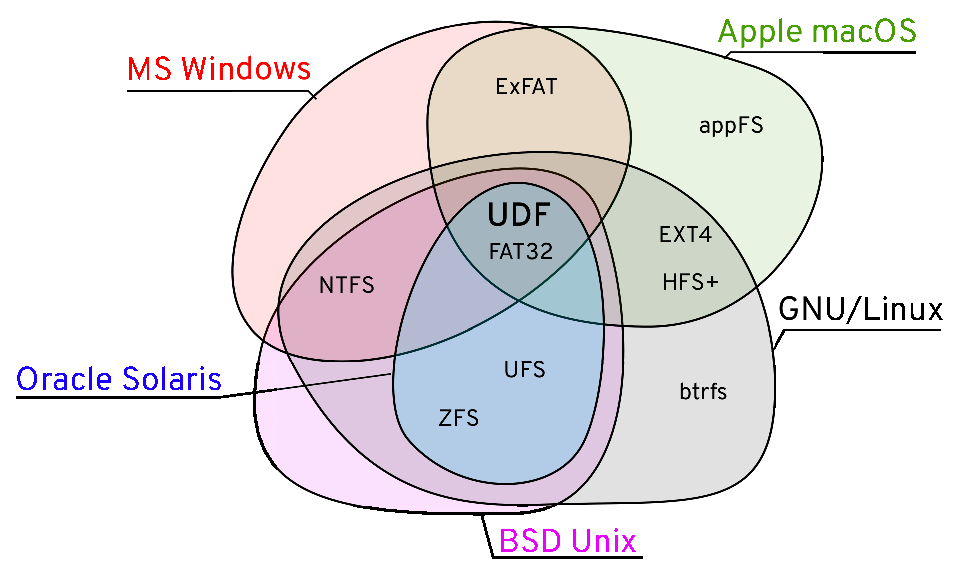
\includegraphics[width=11.5cm]{udf-podpora.eps}
            \end{figure}
		\end{frame}
		\begin{frame}
			\frametitle{Vlastnosti souborového systému UDF}
            \vspace{40pt}
            \begin{itemize}
                \Large\item Souborový systém navržený původně pro optická média,
                \Large\item náhrada zastaralého souborového systému ISO~9660,
                \Large\item vhodný pro přenos dat mezi různými operačními systémy,
                \Large\item multiplatformní od návrhu,
                \Large\item podporovaný v GNU/Linux do verze 2.01 pro zápis (nejnovější verze je 2.60 pouze pro čtení.)
                \Large\item není vhodný jako systémový disk,
                \Large\item neobsahuje žurnál.
            \end{itemize}
        \end{frame}
        \begin{frame}
            \frametitle{Struktura deskriptorů UDF a jejich zabezpečení}
            % TODO popsat deskriptory a jejich zabezpeceni a chyby
			\vspace{40 pt}
			\center
            \begin{figure}
			    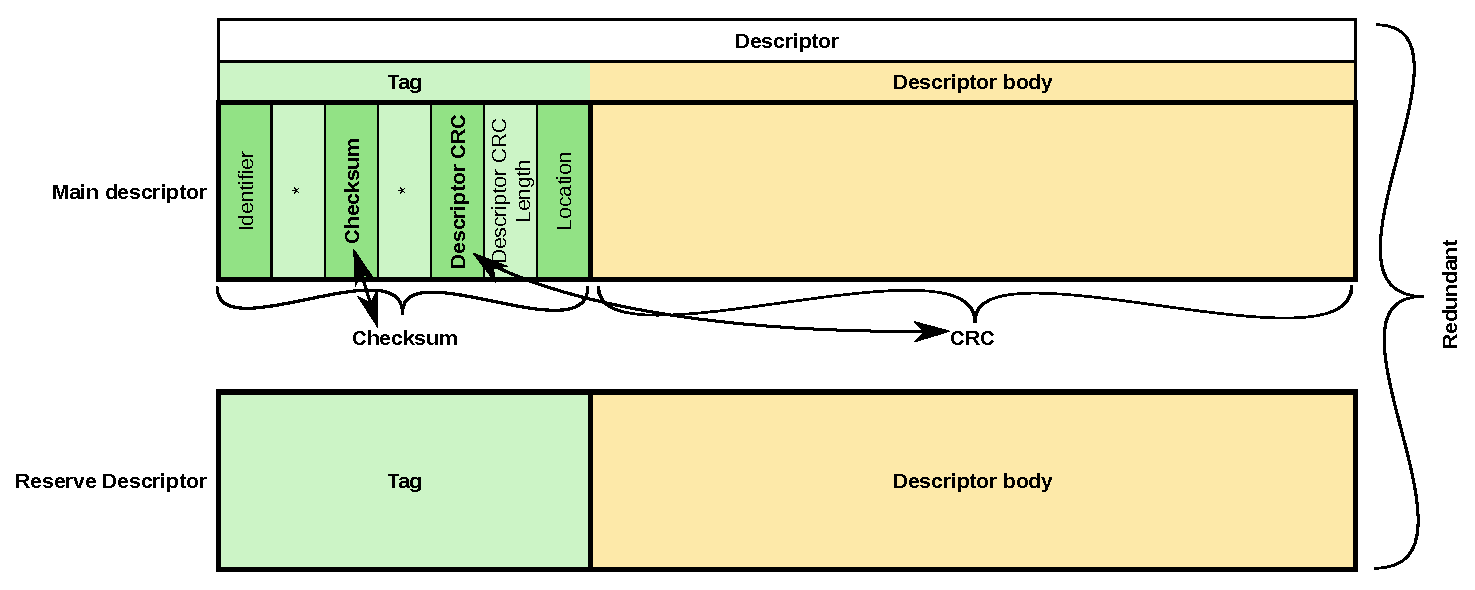
\includegraphics[width=14.5cm]{det-ch.eps}
                \caption{\Large{Zdroj: \cite{udf}, \cite{ecma}}}
            \end{figure}
        \end{frame}
		\begin{frame}
			\frametitle{Struktura souborového systému UDF}
			\vspace{40 pt}
			\center
            \begin{figure}
			    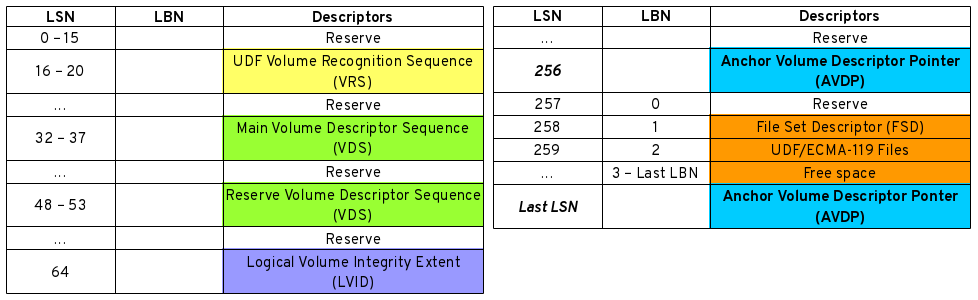
\includegraphics[width=14cm]{strukutra.png}
                \caption{\Large{Struktura souborového systému UDF, zdroj: \cite{udf}, \cite{ecma}}}
            \end{figure}
		\end{frame}
	
    \section{UDF Filesystem Consistency Check}
        \begin{frame}
            \frametitle{Cíl nástroje UDF Filesystem Consistency Check}
            \vspace{30pt}
            \begin{itemize}
                \huge\item Detekovat poruchy na souborovém systému UDF.
                \huge\item Pokud to je možné, poruchy opravit.
                \huge\item Podpora až do standardu UDF 2.01.
            \end{itemize}
        \end{frame}
		\begin{frame}
			\frametitle{Detekovatelné a opravitelné poruchy UDF }
			\vspace{40 pt}
            \begin{itemize}
                \Large\item Poškození každého deskriptoru -- záleží na stupni poškození
                \Large\item Špatné umístění deskriptoru
                \Large\item Nedokončený zápis 
                    \begin{itemize}
                        \large\item Zaalokované místo, ale nezapsaná metadata souboru -- odstranění nedokončeného souboru
                        \large\item Zapsaná metadata i data souboru, ale nenavýšený počet souborů
                        \large\item Zapsaná metadata i data souboru, ale neaktualizovaný počet volných bloků
                        \large\item Vše dokončeno, ale neoznačené dokončení práce na systému
                    \end{itemize}
                \Large\item Špatně nastavené časové značky poslední změny
                \Large\item Nenastavené, duplicitní nebo neshodující se Unique ID každého souboru
%                \Large\item Nenastavené, nebo neshodující se seriové číslo každého tagu (\cmark)
            \end{itemize}
		\end{frame}
        \begin{frame}
            \frametitle{Navržená struktura algoritmu}
            %TODO obrazek s ramecky...
			\vspace{30 pt}
			\center
            \begin{figure}
			    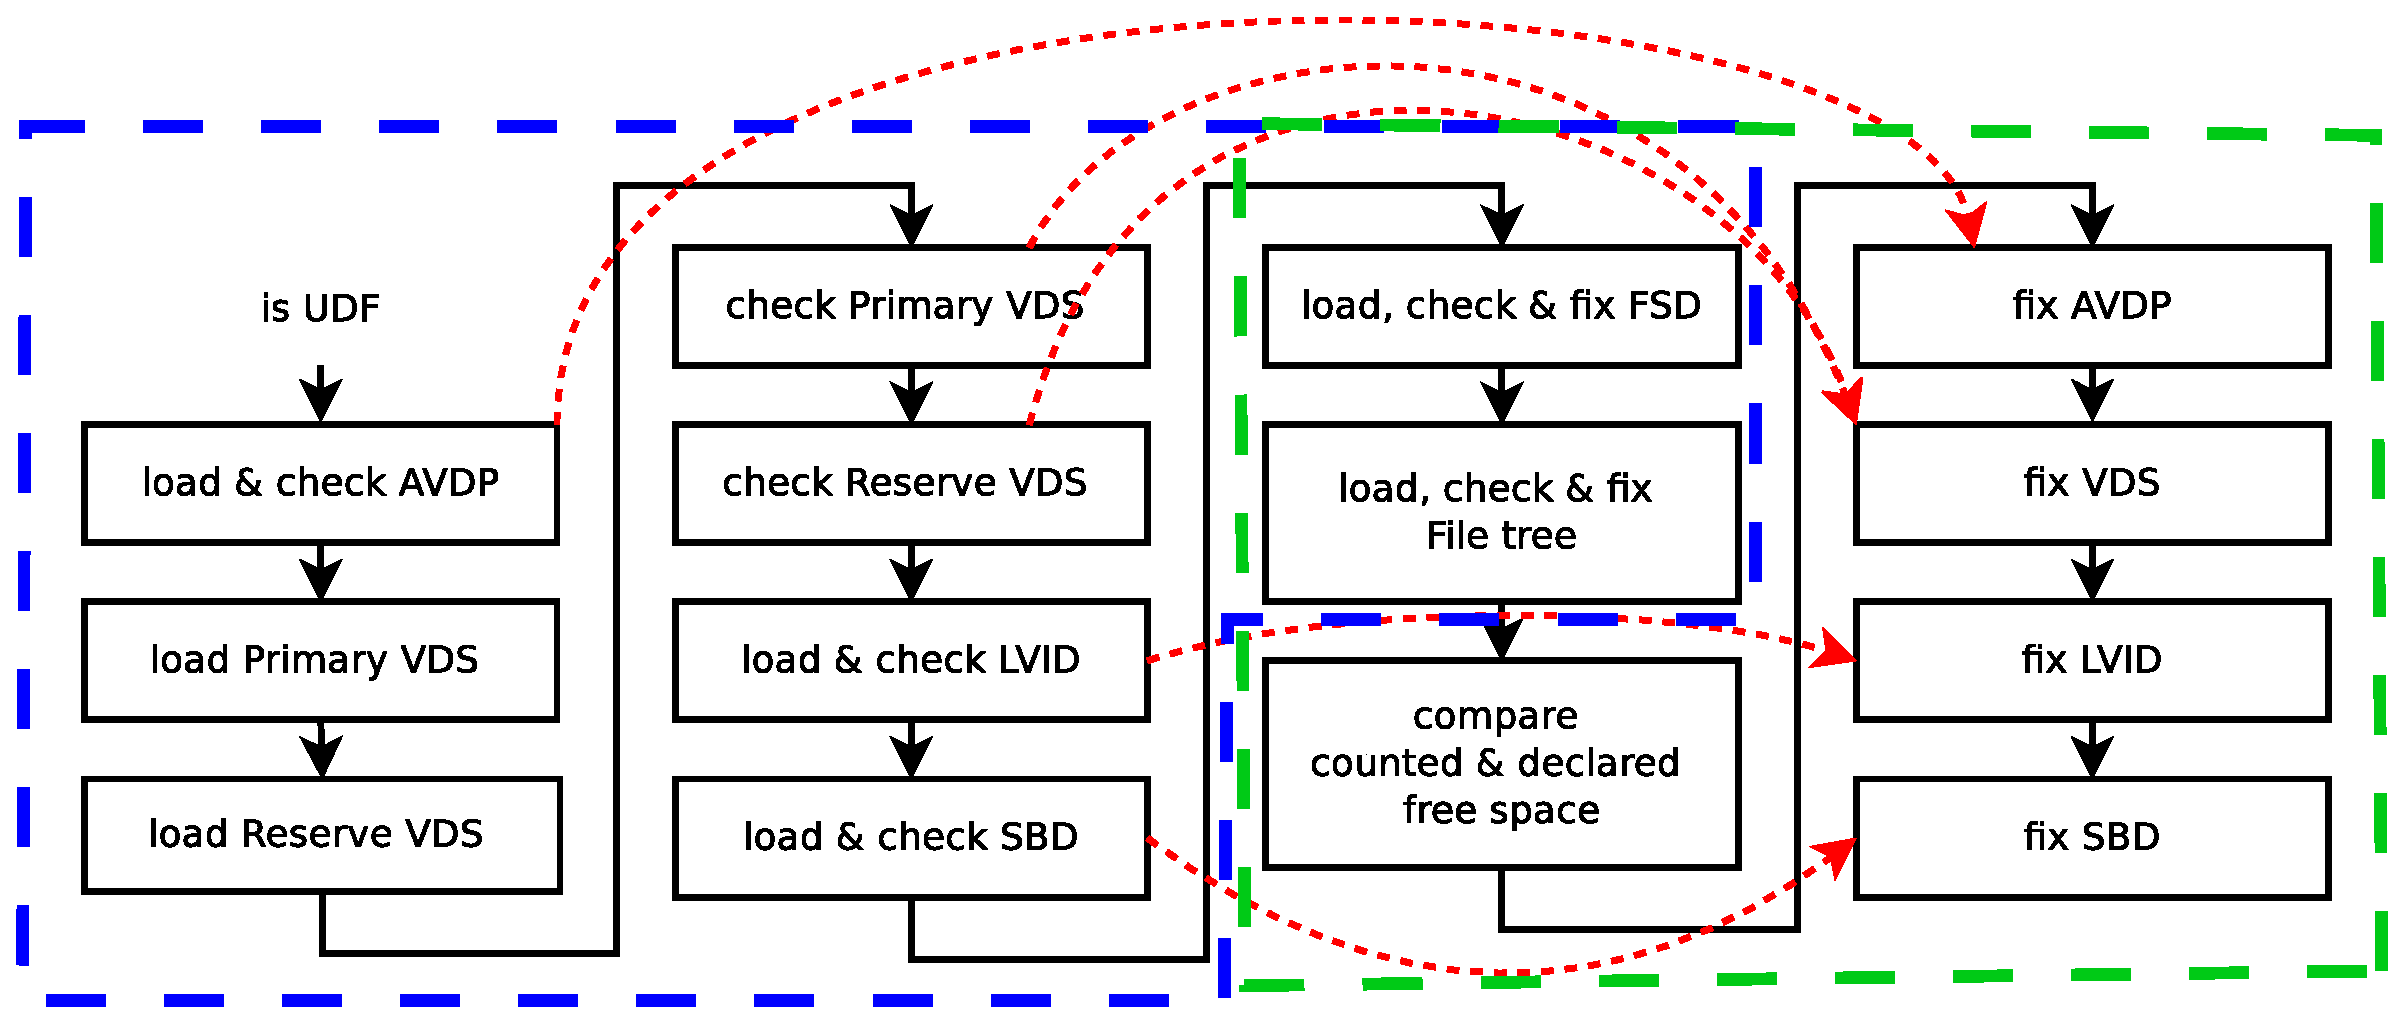
\includegraphics[width=14.8cm]{steps-korekce.eps}
            \end{figure}
        \end{frame}
		\begin{frame}
			\frametitle{Implementace nástroje UDF fsck} % mmap, flock
			\vspace{40 pt}
		    \begin{itemize}
                \Large\item Implementace standardu UDF až do verze 2.01 (stejná jako zbytek balíčku \texttt{udftools})
                \Large\item Realizace je v jazyce C podle standardu C99.
                \Large\item Překlad je zajištěn překladači GCC nebo LLVM, ke správě projektu je použita skupina nástrojů GNU Autotools. Debug byl prováděn pomocí GDB.
            \end{itemize}
		\end{frame}
        \begin{frame}
            \frametitle{Metodika testování a testovací data}
            %TODO popsat testovc9 data
            \vspace{40pt}
            \begin{itemize}
                \Large\item 20~GB testovacích dat ve 32 vzorcích pro automatizované testy.
                \Large\item Pracovní sada testovacích dat použitá při vývoji je řádově větší (přibližně 400~GB dat)
                \Large\item Testy pokrývají všechny aktuálně známé (a automaticky otestovatelné) scénáře.
                \Large\item Testovací prostředí \texttt{cmocka}, které umožňuje tvorbu automatizovaných testů.
                \Large\item Použití služby Travis CI nad těmito daty pro automatický test překladu a zachování funkce.
            \end{itemize}
        \end{frame}

    \section{Závěr}
		\begin{frame}
			\frametitle{Závěr}
			\vspace{40 pt}
			\Large\textbf{Co se podařilo}
			\begin{itemize}
				\item\large Vytvořit open-source nástroj, který je schopný kontrolovat a opravovat poruchy na souborovém systému UDF pro OS Linux.
                \item\large Nástroj byl začleněn do balíčku \texttt{udftools} a bude vydán s příští verzí.
				\item\large Pokrytí standardu UDF až po verzi 2.01.
				\item\large Nástroj je funkční na 32~bitových a 64~bitových little-endian architekturách.
			\end{itemize}
			\Large\textbf{Co je potřeba zlepšit}
			\begin{itemize}
				\item\large Podpora po poslední verzi 2.60 chybí napříč celým balíčkem, udffsck nevyjímaje.
				\item\large Podporu pro big-endian architektury.
			\end{itemize}
			\Large\textbf{Další kroky}
			\begin{itemize}
				\item\large Podpora integračního procesu do linuxových distribucí.
                \item\large Podpora nástroje v budoucnosti.
			\end{itemize}
		\end{frame}
	    
        \begin{frame}
			\frametitle{Zdroje}
			\vspace{40 pt}
            \begin{thebibliography}{9}
                    \setbeamertemplate{bibliography item}[text]
                \bibitem{github} \emph{argorain/udftools. In: GitHub}\/ [online]. 2016 [cit. 2016-11-21]. Dostupné z: \url{https://github.com/argorain/udftools}
                \bibitem{udf} \emph{Universal Disk Format Specification}. Revision 2.01. Cupertino, California: Optical Storage Technology Association, 2000.
                \bibitem{ecma} \emph{ECMA-167}. 3rd Edition. Geneva, Switzerland: ECMA, 1997.
                \bibitem{pali} \emph{pali/udftools. In: GitHub}\/ [online]. 2016 [cit. 2016-11-21]. Dostupné z: \url{https://github.com/pali/udftools}
            \end{thebibliography}
		\end{frame}

		\begin{frame}
			\frametitle{Konec}
			\center
			\vspace{40 pt}
			\Huge\textbf{Děkuji za pozornost.}
		\end{frame}

    \appendix 
    \setcounter{showProgressBar}{0}
        \begin{frame}
            \frametitle{Video ukázka}
            \center
            \large\url{https://www.youtube.com/watch?v=OqRwt0opPp0&t=2s}
        \end{frame}
    \section{Otázky oponenta}
        \begin{frame}
            \frametitle{1. otázka oponenta}
            \vspace{40pt}
            \large
            Jak píšete ve své práci, používá souborový systém UDF pro detekci chyb v deskriptorech současně běžný kontrolní součet kombinovaný s CRC. Myslíte si, že tento způsob je lepší než například použití CRC s delším polynomem popř. použití jednoho CRC pro tag a druhého pro celý deskriptor?
            \vspace{15pt}
            \begin{itemize}
                \item Délka tagu: 16~B, délka těla deskriptoru: 496~B a více
                \item Důvodem rozdělení je urychlení načítání identifikátorů deskriptorů při hledání konkrétního údaje.
                \item Použití kontrolního součtu je pravděpodobně kvůli jeho rychlosti. Na druhou stranu, tag je připravený na 16~bitový kontrolní mechanismus, pokud by to bylo nutné.
            \end{itemize}
        \end{frame}
        \begin{frame}
            \frametitle{2. otázka oponenta}
            \vspace{40pt}
            \large
            Ve čtvrté kapitole se zmiňujete o třech příčinách vzniku chyby na souborovém systému. Jaký máte názor na problematiku „měkkých chyb“ (soft errors), které v některých případech nemusí být detekovány a opraveny řadičem paměťového média. Příklad z praxe - napěťová špička.
            \vspace{15pt}
            \begin{itemize}
                \item Takováto chyba by byla detekována, pokud by dokázala změnit bit v kontrolované oblasti. V tom případě by byl nesprávně nastaven příznak poruchy a došlo by k ,,opravení'' nepoškozeného média. Faktem je, že tento druh chyb není možné na straně fsck kontrolovat a je nutné důvěřovat správnosti přečtených dat, t.j. důvěřovat řadiči, že funguje správně.
            \end{itemize}
        \end{frame}
        \begin{frame}
            \frametitle{Otázka nad rámec zadání}
            \vspace{40pt}
            \large
            (Otázka nad rámec zadání této práce): zvažoval jste možnost kombinace vašeho nástroje, konkrétně jeho modulu určeného pro opravu souborů, s algoritmy používanými nástrojem PhotoRec?
            \vspace{15pt}
            \begin{itemize}
                \item V tuto chvíli ne. Nabízí se otázka vhodnosti kombinace udffsck s PhotRec, vzhledem k rozdílným přístupům k problematice.
                \item udffsck kontroluje a opravuje metadata vs. PhotoRec na základě typických znaků obrázků hledá soubory odpovídající vzoru, t.j. hledá v datech.
            \end{itemize}
        \end{frame}
\end{document}
